\chapter{The LSND and MiniBooNE anomalies}

\minitoc

This chapter will describe experimental apparatus and the results of the LSND and MiniBooNE experiments. The LSND experiment observed an excess of $\bar{\nu}_{e}$ in a primarily $\bar{\nu}_{\mu}$ beam in 2001. The MiniBooNE experiment, built to confirm or rule out the anomaly, observed a significant excess of $\nu_{e}$-like ($\bar{\nu}_{e}$-like) events in a primarily $\nu_{\mu}$ ($\bar{\nu}_{\mu}$) beam. A discussion of the possible physics explanation for the excess will also be provided.

\section{The LSND experiment}
The Liquid Scintillator Neutrino Detector (LSND) was an experiment at the Los Alamos National Laboratory which aimed to detect $\bar{\nu}_e$ in a mainly $\bar{\nu}_{\mu}$ beam, produced with stopping pions. The $\bar{\nu}_e$ interactions were detected via an inverse $\beta$-decay process in the liquid scintillator and tagged with a delayed coincidence between the positron and the subsequent neutron capture, in a fashion similar to the Cowan and Reines experiment. 

LSND found an excess of $\bar{\nu}_e$ interactions, which could be explained as $\bar{\nu}_\mu$ oscillating into $\bar{\nu}_e$ (Figure \ref{fig:resultlsnd}). However, the mass splitting term obtained with LSND data is $\approx1$~eV, one order of magnitude larger than the mass splitting terms obtained with any other reactor, accelerator, atmospheric, or solar experiment \cite{Aguilar:2001ty}. 

A proposed solution to the LSND anomaly is to have one additional neutrino state, which would mix with the standard three neutrinos, in a 3+1 scenario. This fourth neutrino is often called \emph{sterile}, because it does not interact with the $Z$ boson (since its width is compatible only with $N_{\nu}=3$. The PMNS matrix in this case will have an extra dimension ($4\times4$) and the sterile mass neutrino eigenstate will be written as:
\begin{equation}
    \ket{\nu_s}=\sum^{3+1}_{\alpha}U_{i,\alpha}\ket{\nu_{\alpha}}.
\end{equation}
A diagram of the mass hierarchy in this scenario is shown in Figure \ref{fig:masslsnd}.

\begin{figure}
  \begin{subfigure}{0.45\textwidth}
    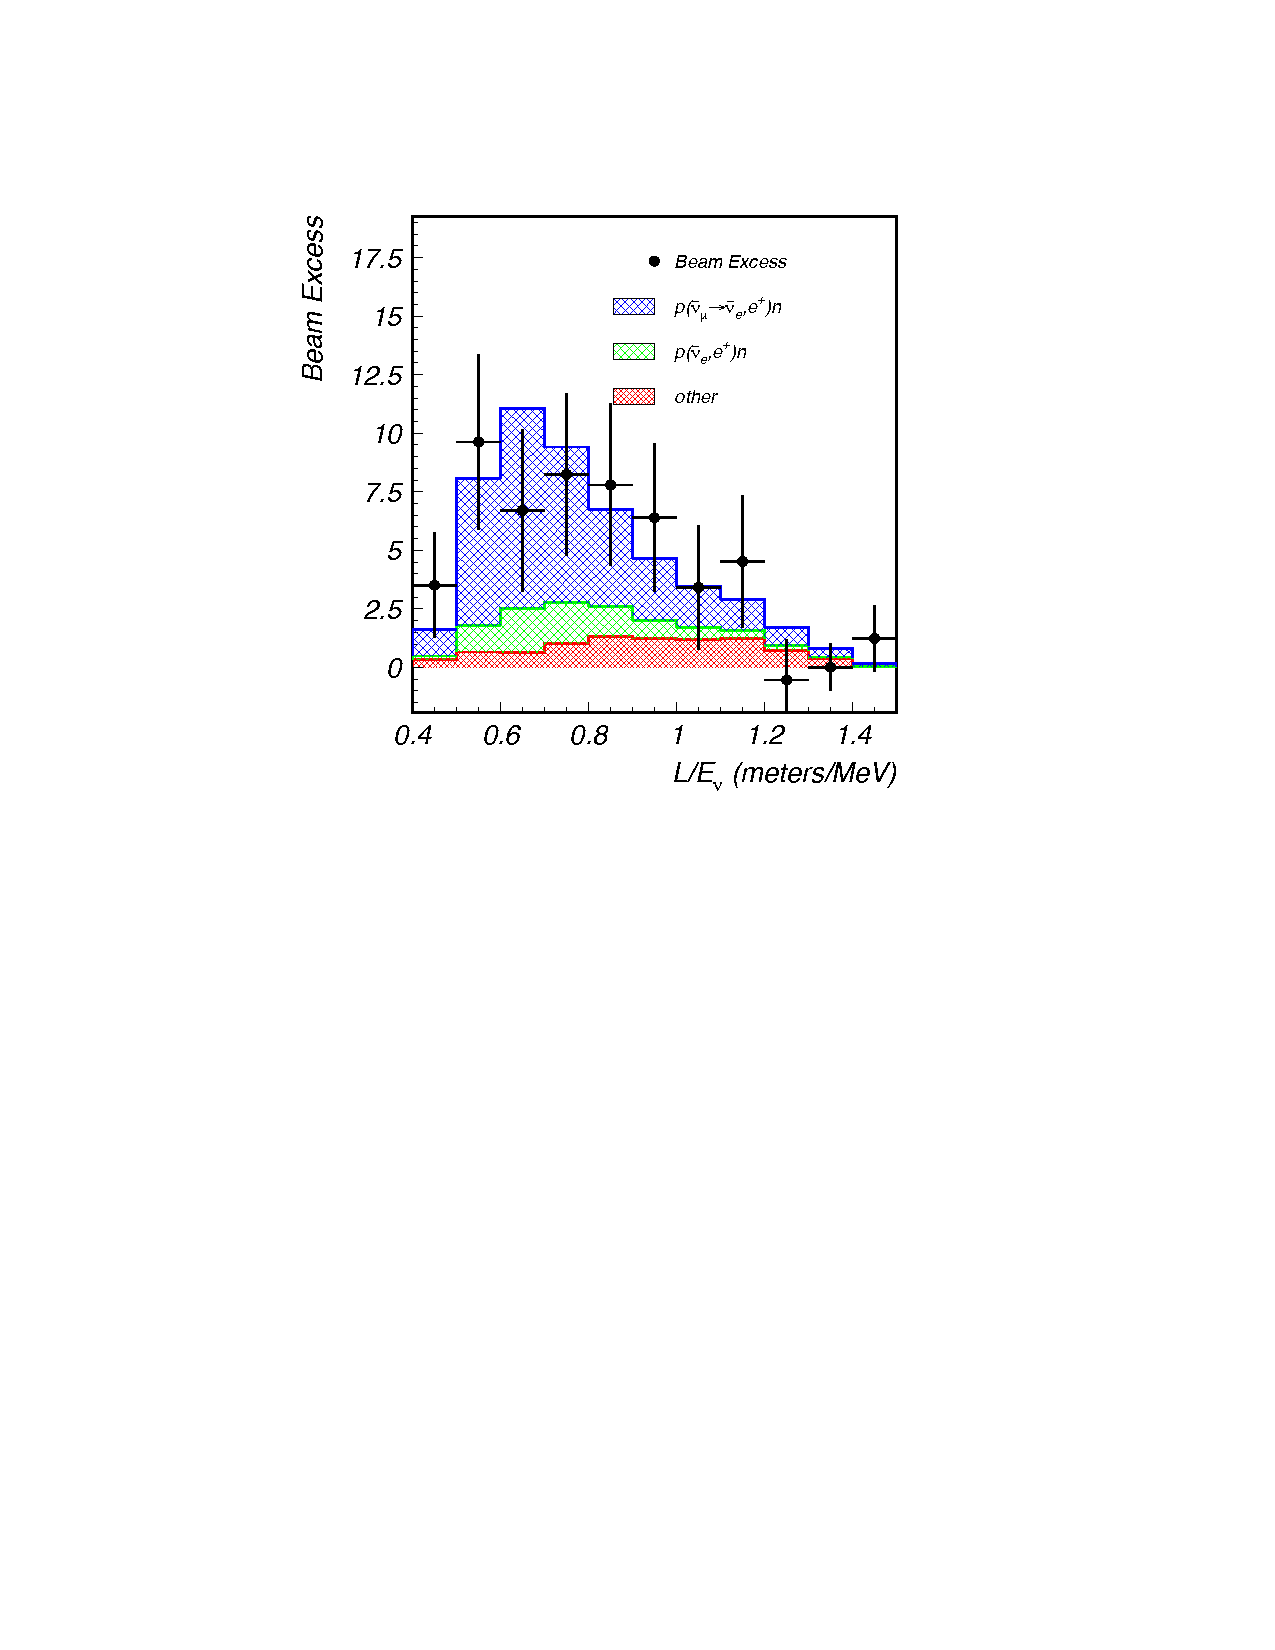
\includegraphics[height=\linewidth]{figures/lsndresult.pdf}
    \caption{$L/E_{\nu}$ distribution for the $\bar{\nu}_{e}$ events in the LSND experiment.}\label{fig:resultlsnd}
  \end{subfigure}\hfill
  \begin{subfigure}{0.45\textwidth}
    \begin{center}
        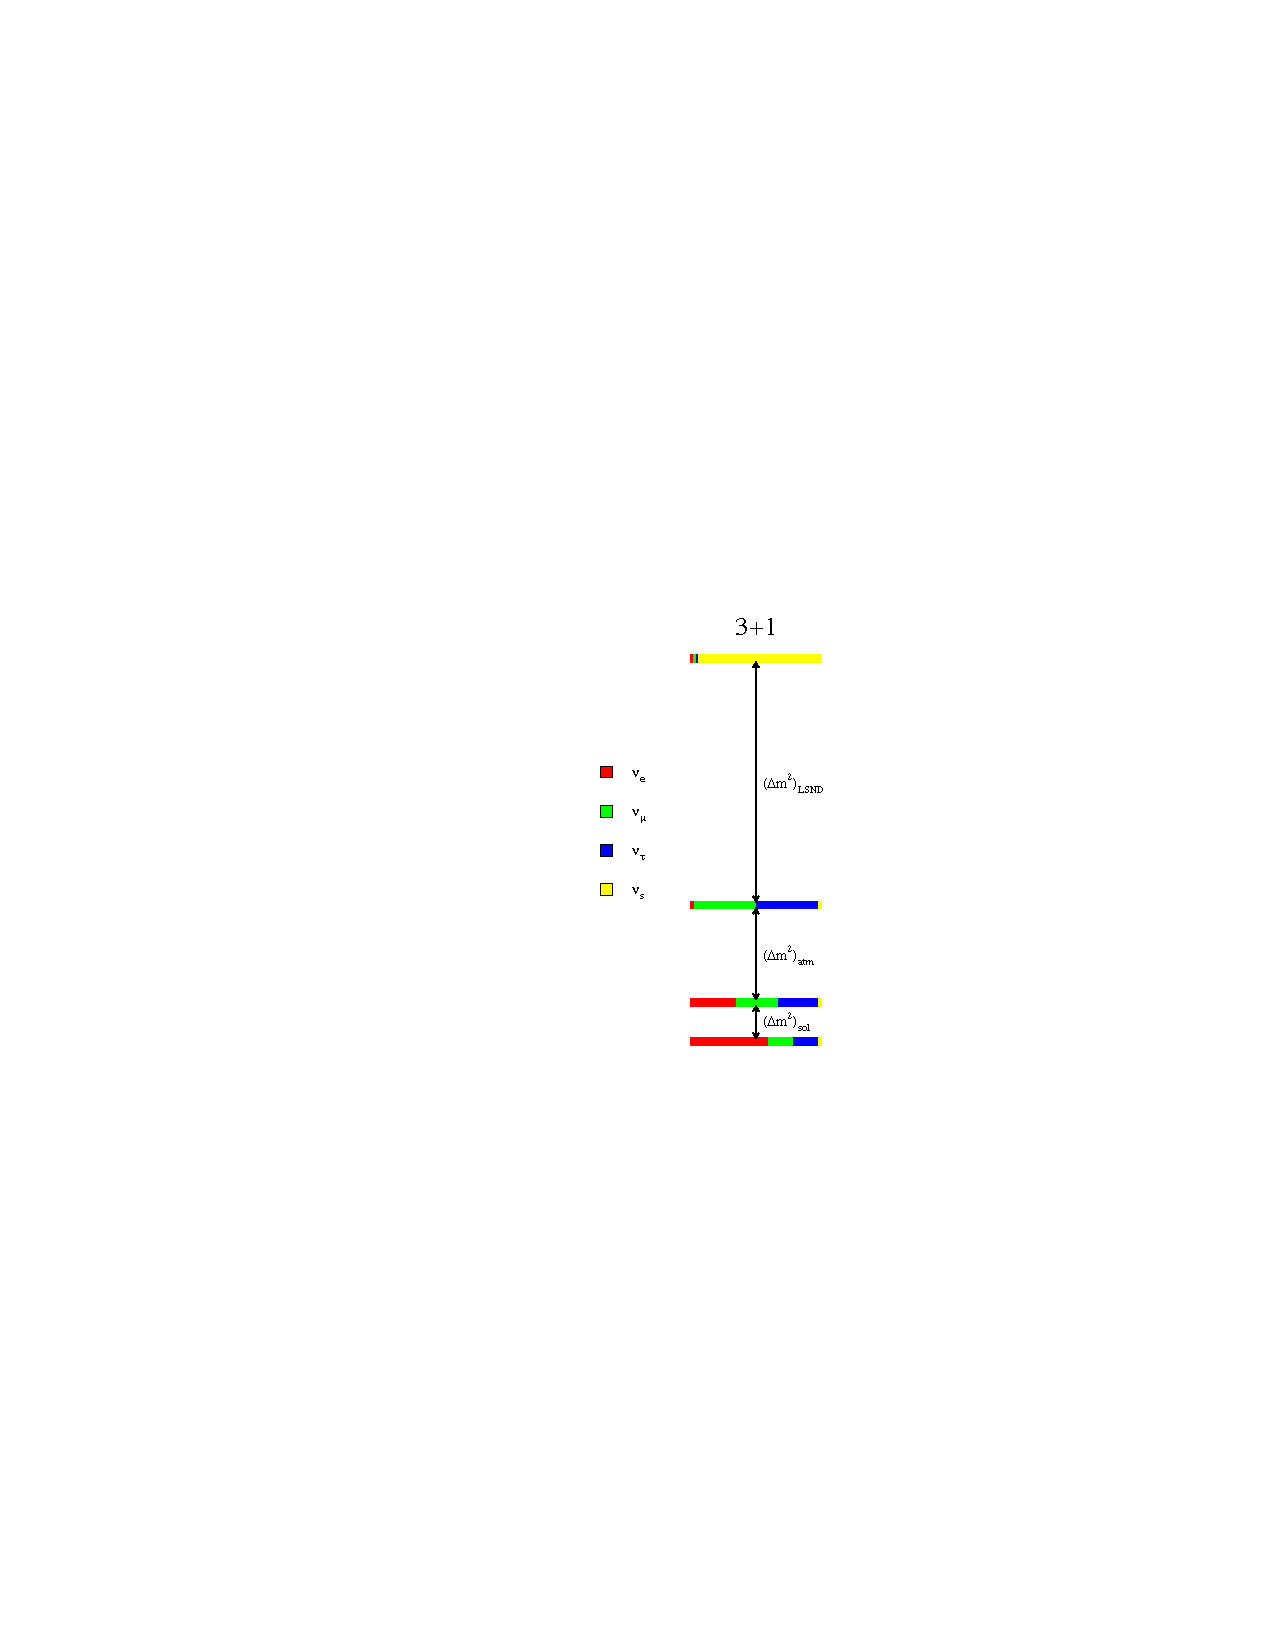
\includegraphics[height=\linewidth]{figures/masslsnd.pdf}
        \caption{Neutrino mass normal hierarchy in the scenario of 3+1 neutrinos.}\label{fig:masslsnd}
    \end{center}
  \end{subfigure}
    \caption{The excess of electron antineutrinos observed by the LSND experiment (left) can be interpreted with the presence of a fourth neutrino state, with a mass splitting term larger than $(\Delta m^2)_{atm}$ and $(\Delta m^2)_{sol}$ (right).}
\end{figure}

Figure \ref{fig:globalfit} shows the global fit of the mixing angles and mass splitting terms using the data coming from the main neutrino detection experiments. It is possible to identify two mass-splitting terms and three mixing angles, compatible with a scenario of 3 neutrino flavours, while the LSND allowed region is clearly exploring a completely different region of the parameter space. 

\begin{figure}[htbp]
    \centering
    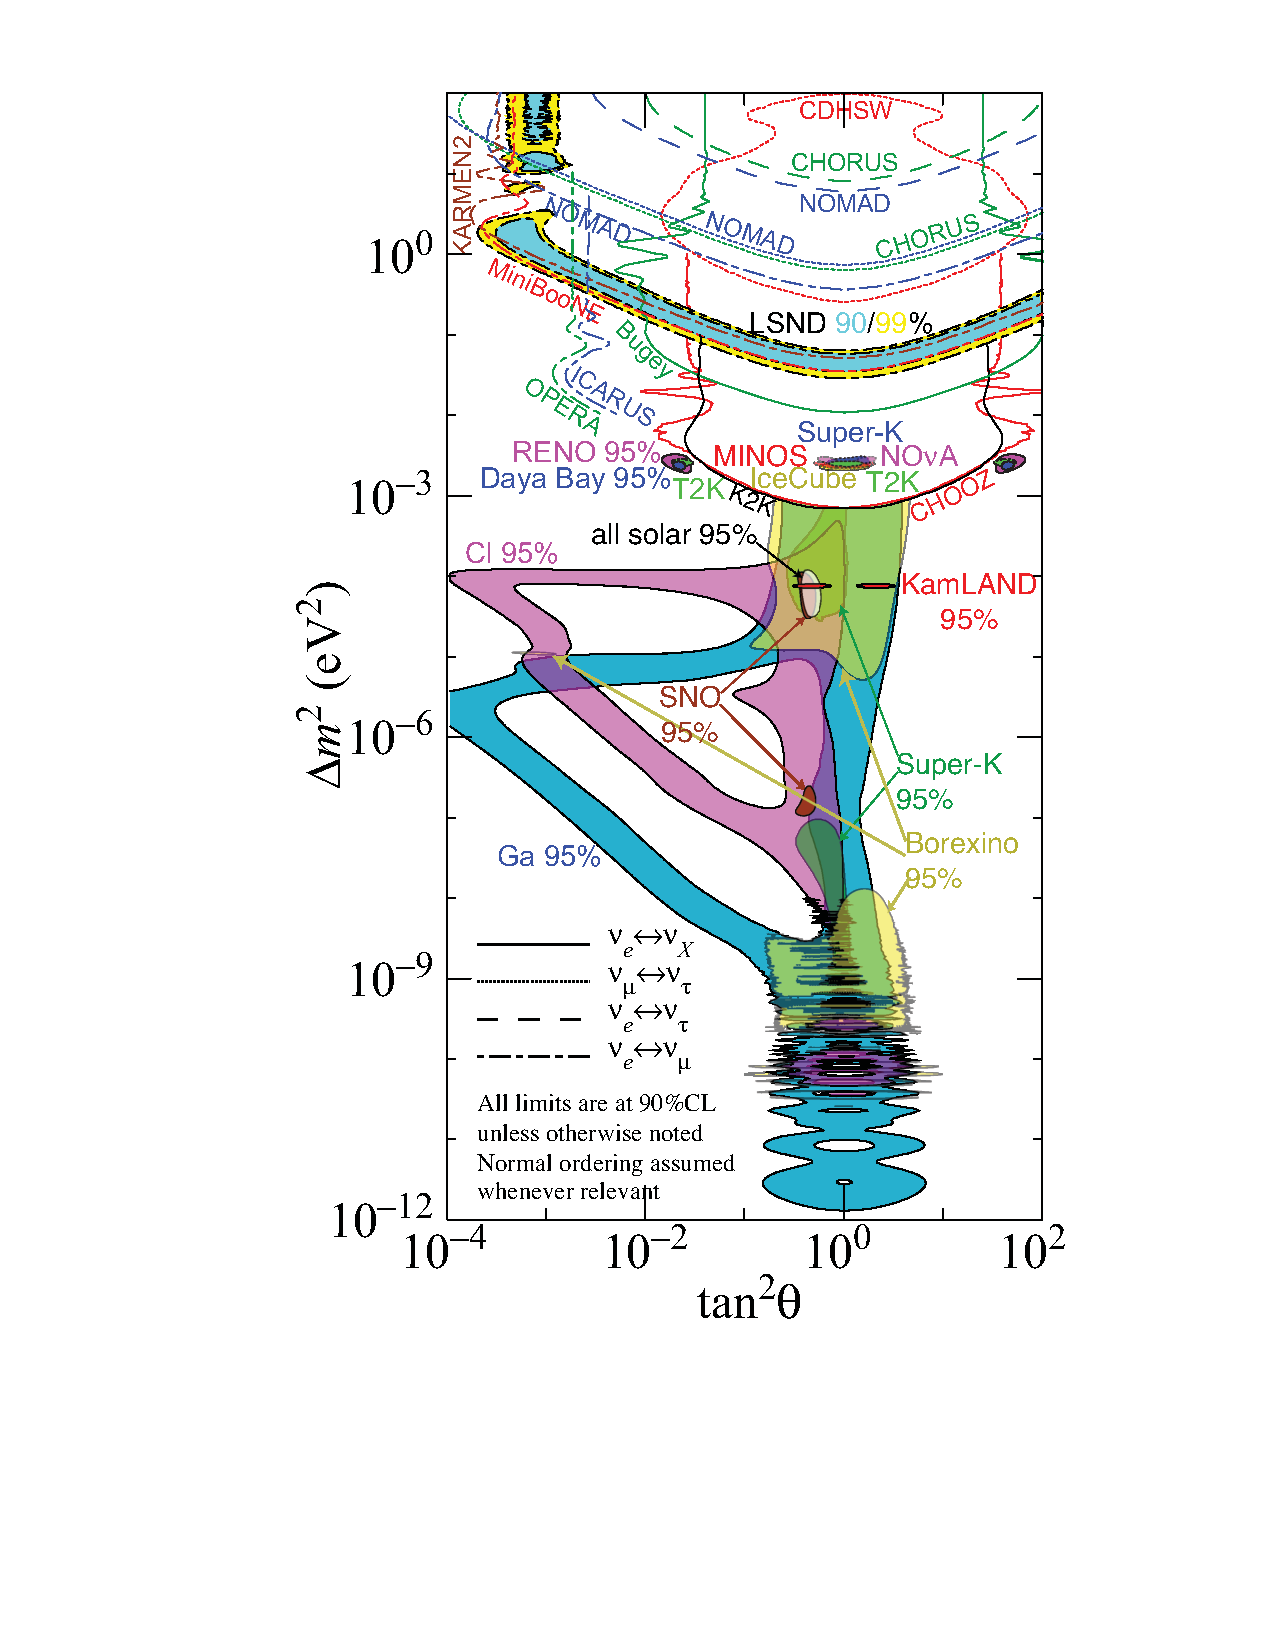
\includegraphics[width=0.7\linewidth]{figures/globalfit.pdf}
    \caption{The squared-mass splittings and mixing angles favored (solid regions) or excluded (open regions) by existing neutrino oscillation measurements. Results are categorized by channels: $\nu_e$ disappearance (solid lines), $\nu_{\mu} \leftrightarrow \nu_{\tau}$  (dotted lines), $\nu_{e} \leftrightarrow \nu_{\tau}$ (dashed lines), and $\nu_{e} \leftrightarrow \nu_{\mu}$ (dashed-dotted lines). The normal mass ordering is assumed where relevant. Adapted from \cite{PhysRevD.98.030001}. Does not include MiniBooNE latest result \cite{Aguilar-Arevalo:2018gpe}.}
    \label{fig:globalfit}
\end{figure}

\section{The MiniBooNE experiment}